\documentclass[11pt]{article}

\usepackage[compact]{titlesec}  
\usepackage{xspace}
\usepackage[margin=0.75in]{geometry}
\usepackage{algorithm}
\usepackage{algorithmicx}
\usepackage{algpseudocode}
\usepackage{amsmath}
\usepackage{graphicx}
\usepackage{pifont} 
% \usepackage{mwe} % new package from Martin scharrer
\usepackage{caption}


\usepackage[colorlinks = true,
            linkcolor = blue,
            urlcolor  = blue,
            citecolor = blue,
            anchorcolor = blue]{hyperref}

\renewcommand{\paragraph}{\vspace{3pt}\noindent\textbf}
\newcommand{\etal}{\textit{et al}.\xspace}
\newcommand{\tick}{\ding{52}} 
\newcommand{\squish}{
  \setlength{\topsep}{0pt}
  \setlength{\itemsep}{0ex}
  %\vspace{-2ex}
  \setlength{\parskip}{0pt}
}

\pagenumbering{roman}
%\newcommand{\codename} {{\sc ICan}\xspace}


\begin{document}
\title{
\vspace{-6ex}
Mirror Mirror on the Wall, \\
 Who is the Most Innovative of Them All? }
\author{Shruti Tople {\footnotesize (A0109720M)} \qquad Shweta Shinde {\footnotesize(A0109685U)} \qquad Loi Luu {\footnotesize(A00095481X)}\\ \texttt{\{shruti90, shweta24, loiluu\}~@comp.nus.edu.sg} \\ \\
Group 6: SSL 3.0
}
\date{}
\bibliographystyle{unsrt}
\maketitle
\pagestyle{empty}
\thispagestyle{empty}

\section{Introduction} 
% 
Innovation is credited with creating the emerging trends in technology. It is
well established and accepted fact that patents play a crucial role in the
study of innovation and technical change~\cite{narin1987patents}. Analyzing
the patent data can help to understand the trends in technology development
and asses the innovation levels of various inventors as well as their
affiliated organizations.

Patent citations allow one to study the importance of individual
patents~\cite{albert1991direct}. The inventor collaboration represents the
state of the innovation environment and the overall contribution of the
organization to the invention field. We focus our study on these two aspect of
the social network of US inventions, and propose metrics to compare the
innovative throughput of a given organization. While doing this, we carefully
account for both the qualitative as well as the quantitative impact of the
organization as a whole thus capturing the enormous heterogeneity in the value
of patents. In this project, we study the inventor and bibliometrics network
of the patents granted by United States Patent and Trademark Office (USPTO).
\section{Problem Description}
\label{sec:prob}
%\subsection{Motivation}

A variety of surveys, reports, and yearly analysis efforts to rank
organizations are based on their innovation. The underlying motive is to measure
which companies and / or products are influencing the market the most.  These
studies consider factors such as the monthly sales, returns, innovation
premiums, royalty earned, the global impact of the innovation, etc. Although,
its crucial to consider the impact of innovation for ranking the
organizations, the metric for such measurement  varies largely across all these 
studies. The consequence is that there is a significant dissonance in the
rankings of all the surveys.  This motivates the need for a standard technique
to compare the innovations on fair grounds and in a holistic way. 

To this end, in this work we argue that patents are one of the main factors for
measuring innovation of an organization and / or an individual. It is true
that patents alone are an insufficient measure to compare the overall
innovation since research papers, consumer products, services are also a major
way of displaying innovation. However, such a measure can be considered as one
of the factors for weighted rankings. Thus, the question is -- given the patent history of
various organizations for past about four decades,  how should one go about in
using this information to measure innovation? Quantifying an abstract
concept such as innovation may not be intuitive and straightforward as it may seem.  

\subsection{Objectives}

To address this challenge, we narrow down our efforts towards tackling
three main  aspects of innovation. Firstly, should the metric purely consider
the quantity of patents filed per unit time (for e.g., month, year, or a
decade) or should it be based on the quality of an invention (for e.g., a
groundbreaking invention such as RSA cryptosystem vs. a insignificant patent
of shapes of chocolates)? Secondly, having a handful of prolific inventors in
an organization may be sufficient to churn patents rapidly, but does it mean
that the organization as a whole is innovative? Lastly, how is the dynamics
between co-inventors, do they tend to collaborate more often with other
impactful inventors, does their involvement affect the frequency and quality 
of patent grant in any way? This helps to throw light on the evolution of 
innovation within an organization, thus giving insights about the future 
prospects of innovation for a given organization.

For a systematic study of the above factors, we confine our problem to
answering the following research questions:

\paragraph{Question 1.} Is an inventor more impactful because he is closely
connected to other impactful inventors in the patent social network? 
%(c)(eigen erdos)

\paragraph{Question  2.} Are inventors closely connected to an impactful
inventor in their own organization or other organizations? %(a) (erdos org)

\paragraph{Question  3.} Has the organization made impactful inventions in
recent past? %(b) (eigen org)


\subsection{Assumptions}
\label{sec:assumptions}
	\begin{itemize}
	\squish
		\item We consider only a subset of the entire patents that were granted till
		date. Specifically, we study patents granted from year 1975 to 2013. There are
		two main reasons for selecting this time frame: (a) Patent data set before
		1975 is only available in OCR format, which is difficult to parse, and
		increases the efforts for preprocessing. (b) The disambiguation
		algorithm~\cite{disambiguation}  requires training models and custom
		parameters, which are available from previous research. However, the models
		and parameters are available only till year 2013, when the study was
		conducted. To maintain the precision in disambiguation and avoid re- running
		the classification on the whole database, we limit our study to patents
		granted till 2013.
		\item We ignore the references to Non-US patents and other sources, since it
		is difficult to track all such sources.  We are only concerned about `Who
		cited this patent?', to decide if it is impactful. In this case, we do not
		need data before 1975, since all the patents after 1975 will be cited only by
		patents after 1975 (for e.g., a patent granted in 2007 will be cited only in
		future i.e., from 2007 onwards.), thus we do not miss any citation data. As
		for the non-US patents and other sources, it is not trivial to track `Who all
		cited this patent outside the patent network?', and this we do not consider
		the non-US and other sources which cite the patents in our dataset.

	\end{itemize}

\subsection{Contributions}

To summarize, we make the following contributions:

	\begin{itemize} 
	\squish
		\item {\em Study the inventor network.} We study various properties of the inventor network in the US grant patent dataset for past four decades.  
		\item {\em Metrics for measuring innovation.} We device a fair metric to measure the innovativeness and impact of an inventor and corresponding organization. This allows us to rank various organizations based on their innovations alone. 
		\item {\em Soundness of metrics.} We verify if our metrics are sound to qualitatively and quantitatively measure the innovation impact of an organization by comparing our ranking results to public lists such as Forbes and Reuters~\cite{forbes, top100}.
	\end{itemize}
\section{Literature review}
% Introduction to patent:
% Patent has a lot of information about innovation, represents the inventive progress of social.
% A good source to study about change and trend in science and technology.
% General research
% Study patent citation to learn about multiple linkage between inventors, organization, firms, etc.
% Economic: relating patent counts to industry & Compustat firms
% Find all distinct inventors and disambiguate them.
% Extract and format patent XML data

\subsection{United States Patent research}

\paragraph{US patent} United States patent database has become widely accessible to researchers and public since the early 1990s. The rich information included in the database cover almost all patents filed in the US in the last four decades. Each patent contains various information about an innovation, together all of them represent the inventive progress of technology and science not only in the US but also around the world~\footnote{In the late 1990s, around 45\% of US patents are awarded to foreign inventors.}. More specially, each patent is highly detailed to cover every
aspect of the invention, enabling us to study the progress from different angles. For example, information included in a patent contains the its belonging technological area, the inventors, the assignee,  terms of fields, types of inventors, citation to another patents, etc.
The database is also a good source to for investigating the change and trend in innovative activity over a particular period of time. 


\paragraph{US patent research analysis} Early research in US patent data goes
back at least to the 1960s when many researchers used patent data in economics
analysis and technology change. For example, in 1966,  Schmookler relates
industries to patent counts~\cite{Schmookler1966}, or in 1982, Griliches
addressed the problem of matching patents to Compustat
firms~\cite{Griliches1982}. The common approach of the early research is that
the rely heavily on the patent counts to come up with some indicative insight.
The simple patent count matrix does not allow them to faithfully capture more
aspects of the information included in each patent and the relation between
patents~\cite{Griliches1987}.

In another line of research, often researchers consider the patent database as
an ``inventor network", in which nodes are inventor or patent, while an edge
represents a citation between patents or a collaboration between two inventors.
Studying this network reveals multiple linkage between inventors,
organizations, firms, regions, etc. In~\cite{Hall01thenber}, Hall~\etal
initiated this line of research by pointing out and addressing several issues
while analysing citation data. They indicated that, due to the drastic change
in the rate of patenting, it is quite challenging to study the {\em received}
citation data of even a small set of patents. The problem is that to collect
all received citations of a particular patent {\em P} granted in year {\em t},
one has to visit all patents granted from year {\em t}. Hall~\etal also propose
two possible approaches to eliminate the problem, we refer the interested
reader to their paper. Using their proposed approaches, they show the main
trends in US patenting activity over three decades by different means of
measurement and across several main technology categories. Many later works
follow Hall~\etal's direction to study different problems in patent
analysing~\cite{Leskovec:2005, Hall2000, leskovec2007graph, Acs2002}.

\paragraph{Extracting and formating data in patent} A general technical problem
when doing patent analysis is how to extract and format data from patent
database. Typically, the data is available in Extensible Markup Language (XML)
format. However, since the patent is often objectively prepared by individual,
thus there is no consistent convention in naming, data field, etc throughout
the data set, thus limiting potential statistical and analytical analysis. For example, if the first student in this report files a patent, her name can be listed as Shruti Tople, or Shruti T., or even Shruti Tople Shrikant, etc. Researchers when processing the data must be aware of these inconsistency and deficiencies to generate a precise and comprehensive results. Recent work has addressed this problem by building a parser which will take account of relevant information into identifying name and/or organization~\cite{formattingpatentdata, disambiguation, Torvik:2009}.
% 
\subsection{Shortest path problem}
Given a graph $G = (V, E)$, we study the problem of finding the shortest path between a source node $u \in V$ and a destination node $v \in V$. In normal graph, the length of a path is the total of nodes along that path. However, in weighted graph where each edge $e_i = (u, v)$ has a weight $w_i$, the length of a path is computed as the total weigh of all edges in the path. For simplicity, we consider the normal graph as the weighted one with all $w_i=1$.

\paragraph{Shortest path from a given vertex} If the source node $u$ is fixed, there exist two popular algorithm to find the shortest path from $u$ to any $v$.
	\begin{itemize}
		\item {\bf Dijkstra algorithm} works only for the graph of non-negative edges. The general idea of Dijkstra algorithm is to find the nearest unvisted node to $u$, namely $k$, at every iteration. After that, the distances of $k$'s neighbors to $u$ are updated based on the distance of $k$ to $u$ and $k$ to that node. The time complexity of the algorithm without/with a min-priority queue are $O(|V|^2)$ and  $O(|E|+|V|\log|V|)$ respectively (where $|V|$ is the number of nodes, $|E|$ is the number of edges).

		One simple trick to make Dijkstra algorithm work with graph having negative edge is as following. Call $w_n < 0$ is the smallest negative weight of an edge in the graph, we add $|w_n|$ to every edge in $G$ to make it a non-negative edge graph $G'$. After that we run Dijkstra algorithm normally on $G'$ and deduct $|w_n|$ from all the edge in the result shortest path to get the correct answer.

		\item {\bf Bellman-ford algorithm} runs slower than Dijkstra algorithm, however it works with graphs having edges of arbitrary weight~\footnote{Note that it is not practical to find a shortest path in a graph having a negative circle.}. The algorithm can also detect the negative circle in the graph. The main insight of Bellman-ford algorithm can be explained in the context of dynamic programing. 		
		The key observation is that any shortest path from $u$ to $v$ in $G$ will have at most $|V|−1$ edges. Thus, we answer the question by sequentially looking for shortest path between $u$ and $v$ which has at most $1, 2, ..., |V|-1$ edges. The algorithm runs in  $O(|V|\cdot |E|)$ time, where $|V|$ and $|E|$ are the number of vertices and edges respectively.
	\end{itemize}

\paragraph{Shortest path between any pair of vertices}
The problem of shortest path between any pair of vertices can be easily solved by running $|V|$ times the above problem of shortest path from a given vertex. The best complexity of such approach is by using Dijkstra algorithm with min-priority queue ($O(|V|\cdot|E|+|V|^2\log|V|)$). We will discuss the other alternatives to address the problem in this section.
	\begin{itemize}	
		\item {\bf Floyd-Warshall algorithm} runs in $O(|V|^3)$. The psudo-code is illustrated in Algorithm~\ref{alg:floyd-war}. The key idea is to improve the estimate distance between $u$ and $v$ by visiting all the nodes and see if the node is in the shortest path between $u$ and $v$.

	 	\item {\bf Johnson algorithm} is more efficient than Floyd-Warshall algorithm when the graph is sparse ($|E| \ll |V|^2$). The algorithm runs in $O(|V|^2\log|V| + |V||E|)$ time. Interested reader can find more details in~\cite{johnson-alg}.
	\end{itemize}

\begin{algorithm}
	\begin{algorithmic}[1]		
		\ForAll{$v \in V$} 
		   \State $dist[v][v] \gets 0$	\Comment{$dist$ is a $|V| \times |V|$ array of minimum distances initialized to infinity}
		\EndFor
		\ForAll{edge $(u,v) \in E$}
		   \State $dist[u][v] \gets w(u,v)$  \Comment{the weight of the edge $(u,v)$}
		\EndFor
		\ForAll{$1 \leq k \leq |V|$}
		    \ForAll{$1 \leq i \leq |V|$}
		      \ForAll{$1 \leq j \leq |V|$}
		         \If {$dist[i][j] > dist[i][k] + dist[k][j]$} 
		            \State $dist[i][j]\gets  dist[i][k] + dist[k][j]$
		        \EndIf
		      \EndFor
		    \EndFor
		\EndFor
	\end{algorithmic}
\caption{Floyd-Warshall algorithm, cited from~\cite{floyd-war-wiki}}
\label{alg:floyd-war}
\end{algorithm}

\subsection{Eigenvector centrality}
\paragraph{Eigenvector centrality} measures the relative centrality of nodes by taking its neighbor nodes into account. The scoring system is designed to differentiate between the connections to a high-scoring node and a low-scoring node, in a sense that connecting to the high-scoring node will make the node more central. Given a graph $G:=(V,E)$ and let $A = (a_{v,t}\in\{0, 1\})$ be the adjacency matrix, the formula to compute the score of a node $v$ is illustrated in Equation~\eqref{eq:eigenvector}

\begin{equation}
	\label{eq:eigenvector}
	x_v = \frac{1}{\lambda} \sum_{t \in M(v)}x_t = \frac{1}{\lambda} \sum_{t \in G} a_{v,t}x_t
\end{equation}
where $M(v)$ is the collection of the neighbors of v and $\lambda$ is a constant called eigenvalue~\cite{Eigenvecto-wiki}.


\paragraph{Katz centrality} A variant of Eigenvector centrality is Katz centrality, which computes a node score also by taking influence of other nodes into account. In this case, the distance from all other nodes are considered, and the larger the distance between $u, v$, the smaller the influence that $u$ and $v$ have on each other. Interested readers are referred to~\cite{katz-wiki} for more details.

\paragraph{Pagerank algorithm} Another variant of Eigenvector centrality is PageRank used by Google Search~\cite{pagerank-wiki} to rank the websites in their search results. The difference between Pagerank and Eigenvector centrality and Katz centrality is that the connecting neighbors are taken into account, not the connected nodes. For example, in Eigenvector centrality, all nodes $v$ so that $a_{u, v}= 1$ will have affect on $u$'s score, while in Pagerank, only nodes $v$ having $a_{v, u} = 1$ will do.

\section{Data Collection}

\subsection{Pre-processing}

\begin{figure}[H]
		  \centering	
          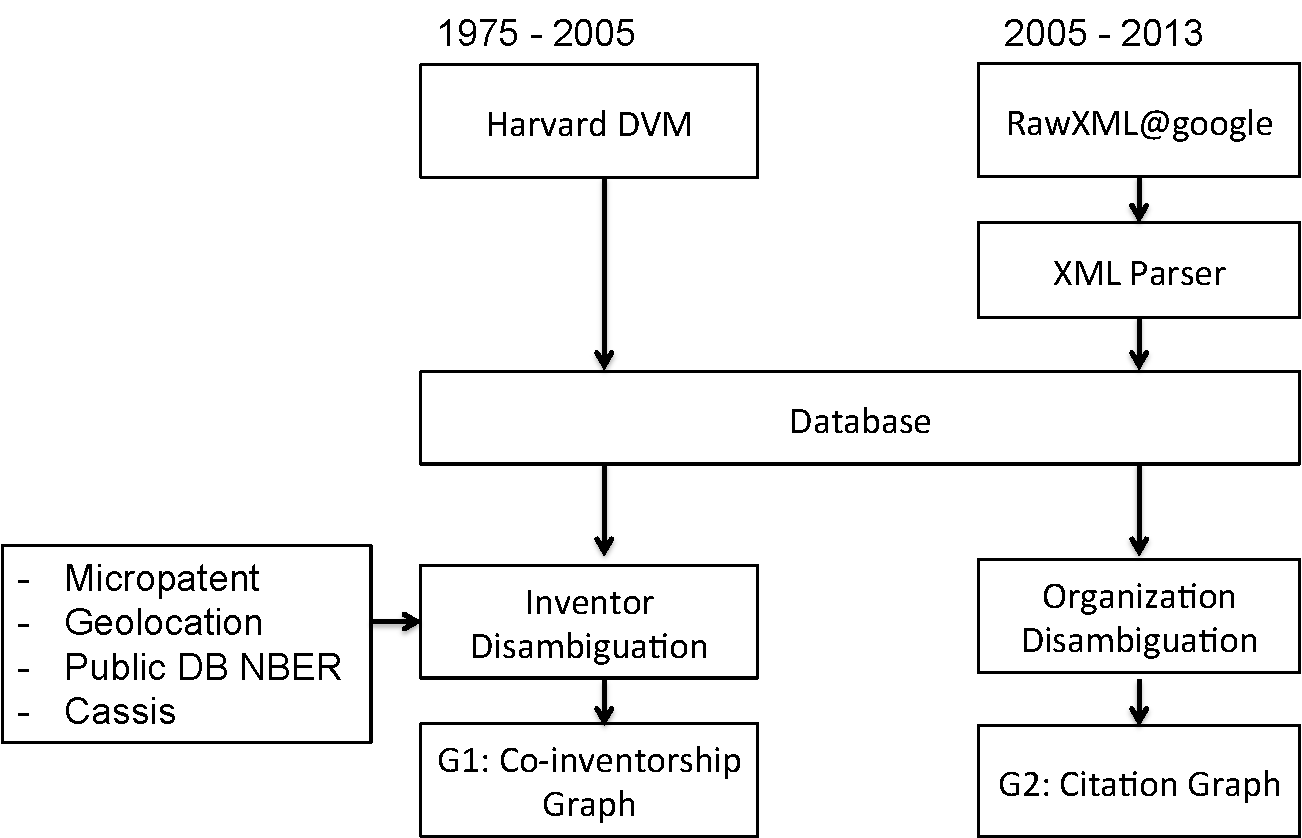
\includegraphics[scale=0.6]{../figures/process.pdf}
          \caption{This is the second figure}
\end{figure}

\subsection{Author Disambiguation}

\subsection{Organisation Disambiguation}

\begin{table*}[h] 
  \centering
  \begin{tabular}{@{}c@{}} 

  \begin{minipage}{0.25\linewidth}

\begin{lstlisting}[]
<node id="n196819">
  <data key="Loc">BOZEMAN-MT-US</data>
  <data key="Name">BERG, LLOYD</data>
  <data key="id">04292142-1</data>
  <data key="Patents">247</data>
</node>
\end{lstlisting}

  \end{minipage}
  \hspace{0.05\linewidth}
  \begin{minipage}{0.3\linewidth}

\begin{lstlisting}[]
<node id="n471405">
  <data key="Loc">BOZEMAN-MT-US</data>
  <data key="Name">EDISON, THOMAS A</data>
  <data key="id">05147512-2</data>
  <data key="Patents">1</data>
</node>
\end{lstlisting}

  \end{minipage}
  \hspace{0.05\linewidth}
  \begin{minipage}{0.3\linewidth}

\begin{lstlisting}[]
<edge source="n196819" target="n471405">
  <data key="tId">05147512-2</data>
  <data key="hId">04292142-1</data>
  <data key="AppYear">1991</data>
  <data key="Weight">1</data>
</edge>



\end{lstlisting}

  \end{minipage}
  
  \end{tabular}

\label{listing}
\caption{\footnotesize Snippet from GraphXML. Shows the nodes for Lloyd Berg and Thomas Edison and the corrsponding edge between them.}
\end{table*}
\section{Solution Approach}
\label{sec:sol}
With our problem definition narrowed down to three sub-questions, we build a social graph model to address these research questions. 
After we have the social graph, we select the appropriate network metrics to measure the aspects of innovation.
With these metrics, we can answer the research questions as well as provide empirical evidence to verify our rankings.

\subsection{Inventor Network Model}
\label{sec:model}
Our social graph models two aspects of the inventor network:  `Which inventors
and organizations have joint patents?' and `How many patents cite a certain
patent?'. These two networks abstracts out just enough information to address
our three sub-problems discussed in Section~\ref{sec:prob}. We describe our graph models in detail below:

\paragraph{Graph G1: Co-inventorship Graph}

	\begin{itemize}
	\squish
		\item {Vertices:} Inventors  ($I_1$, $I_2$, ...)
		\item {Edges:} Signify co-inventorship on one / more patents
	\end{itemize}

There exists an edge between $I_1$ and $I_2$ if these two inventors have a
joint patent. Since two inventors can have multiple joint patents, the weight
signifies the number of joint patents

\paragraph{Graph G2: Citation Graph.}

	\begin{itemize}
	\squish
		\item {Vertices:} Patents ($P_1$, $P_2$, ...)
		\item {Edges:} Citations 
	\end{itemize}

There exists a directed `citation' edge from $P_1$ to $P_2$ if $P_1$ cites $P_2$.

\subsection{Definitions \& Insights}

	\begin{itemize}
	\squish
		\item {\em Collaborative distance.} For any two inventors, we define
		the collaborative distance as the length of the shortest path in
		Graph G1.
		\item {\em Invention impact.} For a given inventor / organization, we define his /
		her invention impact as the sum of degree centrality for
		all the patents from Graph G2 of this inventor / organization.
	\end{itemize}

% \subsection{Insight}

In our model, the impact of an inventor is measured by the total number of citations
to the patents that he / she invents. Thus, intuitively, the more is the sum of degree
centrality measure, the inventor is more `impactful'. Similarly, we use
collaborative distance to measure the `connectedness' between two inventors.
Thus, intuitively, the smaller the collaborative distance, the closer they are
to each other in terms of connection in the graph.  In a nutshell, the answers
to our questions framed in our problem description follow from these insights:

\paragraph{Answer 1.} Check the correlation between collaborative distance and invention impact.
If inventors with smaller value of collaborative distance from an impactful inventor have 
high value for invention impact, then we can say that collaborative distance from an impactful inventor
affects the invention impact of an individual inventor.

\paragraph{Answer 2.} Check the correlation between collaborative distance and organization.
Check whether most inventors within the same organization as the impactful inventor
have smaller collaborative distance or inventors outside the orgranization have
smaller distance.

\paragraph{Answer 3.} Check the correlation between invention impact and organization.
Calculate the sum of degree centralities from Graph G2 for each organization and rank the 
organization depending on the centrality measure. Organization with highest sum of degree
centralities is the most impactful and is ranked one. Compare this list with publicly available
list of innovative organization. Similarity in the two list indicates that total citations for the patents
is a correct metric to decide the invention impact of an organization.



\section{Project Progress and Plan}


\subsection{Progress}

%discuss why we swapped 2 and 3
	\begin{itemize}

		\item {\em Data Processing:} We extract the data from raw XML to SQL and GraphML format for years 2005 to 2013, for the rest of the data, we relied on the already available processed data from Harvard.

		\item {\em Inventor Disambiguation:} We used the previously proposed pre-processing and disambiguation algorithm to
		generate a list of unique inventors.  

		\item {\em Evaluation Phase I - Collaborative Distance:} We calculated the shortest path of each inventor w.r.t
		to Thomas Edison. We used three algorithms viz. Djikstra, Bellman-Ford,	Johnson from IGraph to do this.
		We also analyzed their scalability with respect to the invention network graph and compared their performance.

		\item {\em Social Network Behavior:} Computed the distribution of the collaborative distance w.r.t. Thomas Edison for our network, and also studied if the overall network follows power law for various popularity measures.
	\end{itemize}

\subsection{Plan}

	\begin{itemize}
	%\squish
		\item {\em Organization / Assignee Disambiguation:} For the next phase of evaluation, we will run a simple pre-processing
		algorithm for disambiguating organization names. For example, IBM Corp. vs. International Business Machines Corporation are considered different organizations currently. We will use a similar algorithm as for inventor disambiguation, to merge multiple assignees with such names into a single entity.

		\item {\em Evaluation Phase II - Eigenvalue centrality:} Use the Newman's leading eigenvector
		algorithm in IGraph to calculate eigenvalue centrality for each unique
		inventor with respect to patents that cite his / her patent. In this case, we do not need data before 1975, since all the patents after 1975 will be cited only by patents after 1975 (for e.g., a patent granted in 2007 will be cited only in future i.e., from 2007 onwards.), thus we do not miss any citation data.  

		\item {\em Data analysis and comparison:} Plot the graphs for the above
		generated data and analyze the relationship between the above two
		measurements. Compare our ranking results for the most innovative organization with publicly
		available list such as Forbes list, to check if our ranking metric coincides
		with the results of other metrics.
	\end{itemize}

\begin{table}[H]
%\footnotesize
\centering
\begin{tabular}{| l | l | l |}
\hline
{Date} & {Activity} & Progress \\
\hline
\hline
24th March & Data Extraction and Author Disambiguation & \tick \\
31st March & Calculate Eigenvalue centrality for all nodes & - \\
7th April & Calculate shortest path between nodes - Run 3 algorithms & \tick \\
14th April &  Comparison charts and analysis & - \\
17th April & Final Report Submission & - \\
\hline
\end{tabular}
\label{tbl:milestone}
% \vspace{-0.5cm}
\end{table}
\section{Implementation \& Evaluation}
\label{sec:eval}


We describe in detail our implementation method and evaluation procedure for
answering  our goals using the patent dataset. 

\subsection{Analysis Tools and Platform}


	\begin{itemize}
		\squish
		\item We use IGraph for all our graph analysis and metric
		calculation~\cite{gephi, igraph}. Table~\ref{tab:model} gives the details
		about Graph G1 in terms of its total number of nodes , edges , patents, the
		source node  of the graph and the average distance between the source node and
		all other nodes .    We choose Kia Silverbrook as our source node as he is one
		of the top and popular inventors in the patent dataset with maximum number of
		patents. We calculate the shortest path of all other nodes from Kia Silverbrook.
		We run three algorithms particularly Djikstra shortest path algorithm,
		Bellman-ford and Johnson available in IGraph tool on our Graph G1.
		\item The configuration of our experimental desktop machine is RAM $32$ GB, $12$
		core with processor speed of $2.6$ GHz Intel® Xeon(R) CPU E5-2630 v2 and platform is Ubuntu $14.04$.
	\end{itemize}

\begin{table*}[t]
\centering
\begin{tabular}{clcl}
\hline
\multicolumn{1}{|l|}{\textbf{Rank}} & \multicolumn{1}{l|}{\textbf{Organization Name}}                  & \multicolumn{1}{l|}{\textbf{Rank}} & \multicolumn{1}{l|}{\textbf{Organization}}                     \\ \hline
\multicolumn{1}{|c|}{1}             & \multicolumn{1}{l|}{International Business Machines Corporation} & \multicolumn{1}{c|}{11}            & \multicolumn{1}{l|}{Hewlett Packard Company}                   \\ \hline
\multicolumn{1}{|c|}{2}             & \multicolumn{1}{l|}{Hitachi Ltd}                                 & \multicolumn{1}{c|}{12}            & \multicolumn{1}{l|}{Texas Instruments Incorporated}            \\ \hline
\multicolumn{1}{|c|}{3}             & \multicolumn{1}{l|}{Matsushita Electric Industrial Co Ltd,}      & \multicolumn{1}{c|}{13}            & \multicolumn{1}{l|}{Sony Corporation}                          \\ \hline
\multicolumn{1}{|c|}{4}             & \multicolumn{1}{l|}{Canon Kabushiki Kaisha,}                     & \multicolumn{1}{c|}{14}            & \multicolumn{1}{l|}{Intel Corporation}                         \\ \hline
\multicolumn{1}{|c|}{5}             & \multicolumn{1}{l|}{Motorola Inc,}                               & \multicolumn{1}{c|}{15}            & \multicolumn{1}{l|}{Micron Electric Co Ltd}                    \\ \hline
\multicolumn{1}{|c|}{6}             & \multicolumn{1}{l|}{Toshiba Corporation,}                        & \multicolumn{1}{c|}{16}            & \multicolumn{1}{l|}{Eastman Kodak Company}                     \\ \hline
\multicolumn{1}{|c|}{7}             & \multicolumn{1}{l|}{General Electric Company,}                   & \multicolumn{1}{c|}{17}            & \multicolumn{1}{l|}{Minnesota Mining \& Manufacturing Company} \\ \hline
\multicolumn{1}{|c|}{8}             & \multicolumn{1}{l|}{AT\&T Corp,}                                 & \multicolumn{1}{c|}{18}            & \multicolumn{1}{l|}{Microsoft Corporation}                     \\ \hline
\multicolumn{1}{|c|}{9}             & \multicolumn{1}{l|}{Fujitsu Limited,}                            & \multicolumn{1}{c|}{19}            & \multicolumn{1}{l|}{Samsung Electronics Co Ltd}                \\ \hline
\multicolumn{1}{|c|}{10}            & \multicolumn{1}{l|}{Xerox Corporation,}                          & \multicolumn{1}{c|}{20}            & \multicolumn{1}{l|}{NEC Corporation}                           \\ \hline                                                               
\end{tabular}
\caption{List of top 20 innovators for year 2013 as calculated by our proposed metrics.}
\label{lst:top20}
\end{table*}

\subsection{Evaluation Steps}
	\begin{itemize}
		\squish
		\item {\em Evaluation Phase I - Collaborative Distance:} We calculated the 
		shortest path of each inventor w.r.t to Kia Silverbrook. We used three
		algorithms viz. Djikstra, Bellman-Ford, Johnson from IGraph to do this. We
		also analyzed their scalability with respect to the invention network graph
		and compared their performance.
		\item {\em Social Network Behavior:} Computed the distribution of the 
		collaborative distance w.r.t. Kia Silverbrook for our network, and also studied
		if the overall network follows power law for various popularity measures.
		\item {\em Evaluation Phase II - Degree centrality:} Use the in-built
		algorithm in IGraph to calculate degree centrality
		for each unique inventor and organization with respect to patents that cite his / her patent.
		\item {\em Data analysis and comparison:} Plot the graphs for the above
		generated data and analyze the relationship between the above two
		measurements. Compare our ranking results for the most innovative organization
		with publicly available list such as Reuters list, to check if our ranking
		metric coincides with the results of other metrics.
	\end{itemize}



\subsection{Results}

\paragraph{Answer 1.}
We first calculate the total number of citations for each inventor from Graph G2. Using the collaboration distance calculated from G1, we plot a graph of distance (connectedness) vs. total number of citations (invention impact) of each inventor. 
Figure~\ref{fig:distance_citation} shows the relation of the distance from
Kia Silverbrook and the no. of total citations for an inventor. This graph gives a positive answers our Question 1: 
Yes, an inventor is more impactful because he is closely
connected to other impactful inventors in the patent social network.

\begin{figure}[t]
  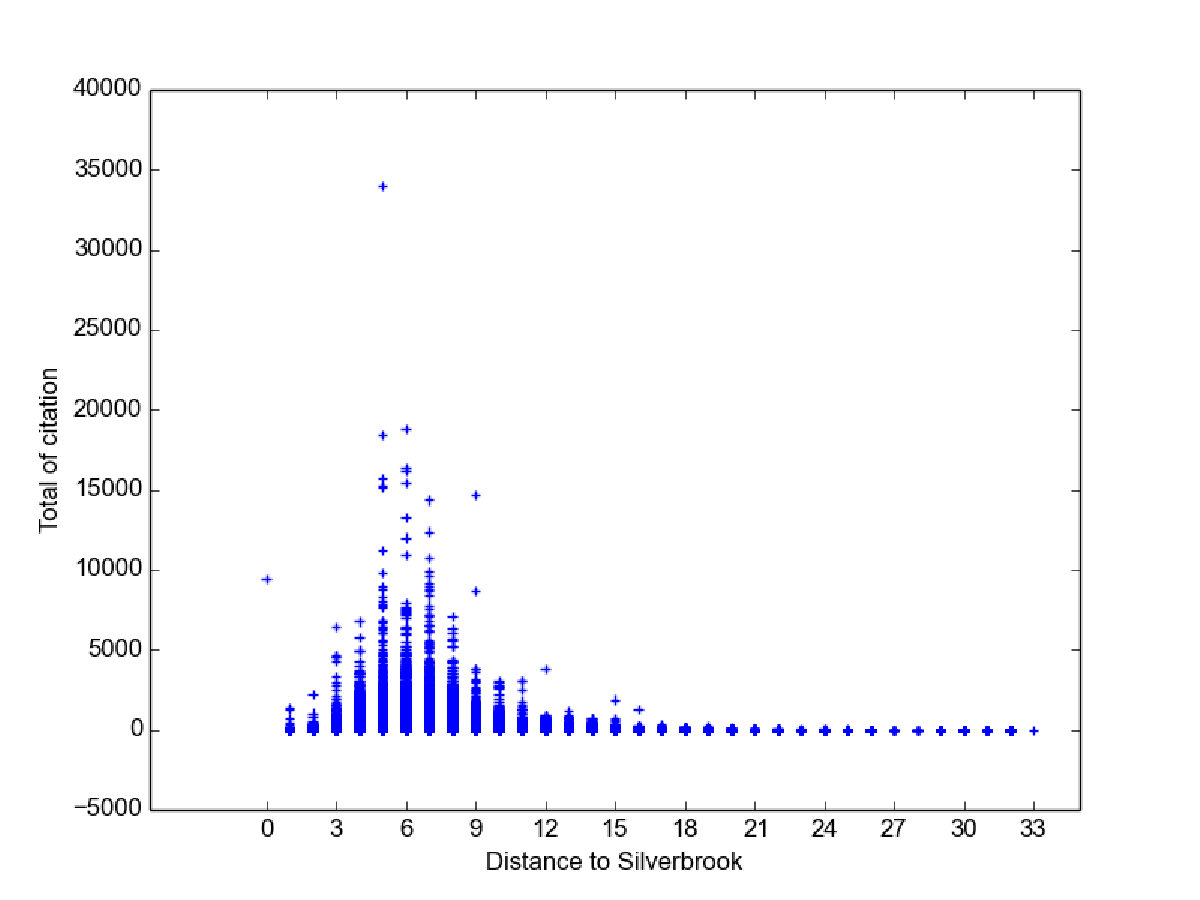
\includegraphics[scale=0.425]{figure/abc.pdf}
  \caption{ Relationship graph of no. of citations for all patents of an inventor (i.e., the cumulative degree centrality) and his distance from Kia Silverbrook}
\label{fig:distance_citation}
\end{figure}
\begin{figure}[t]
  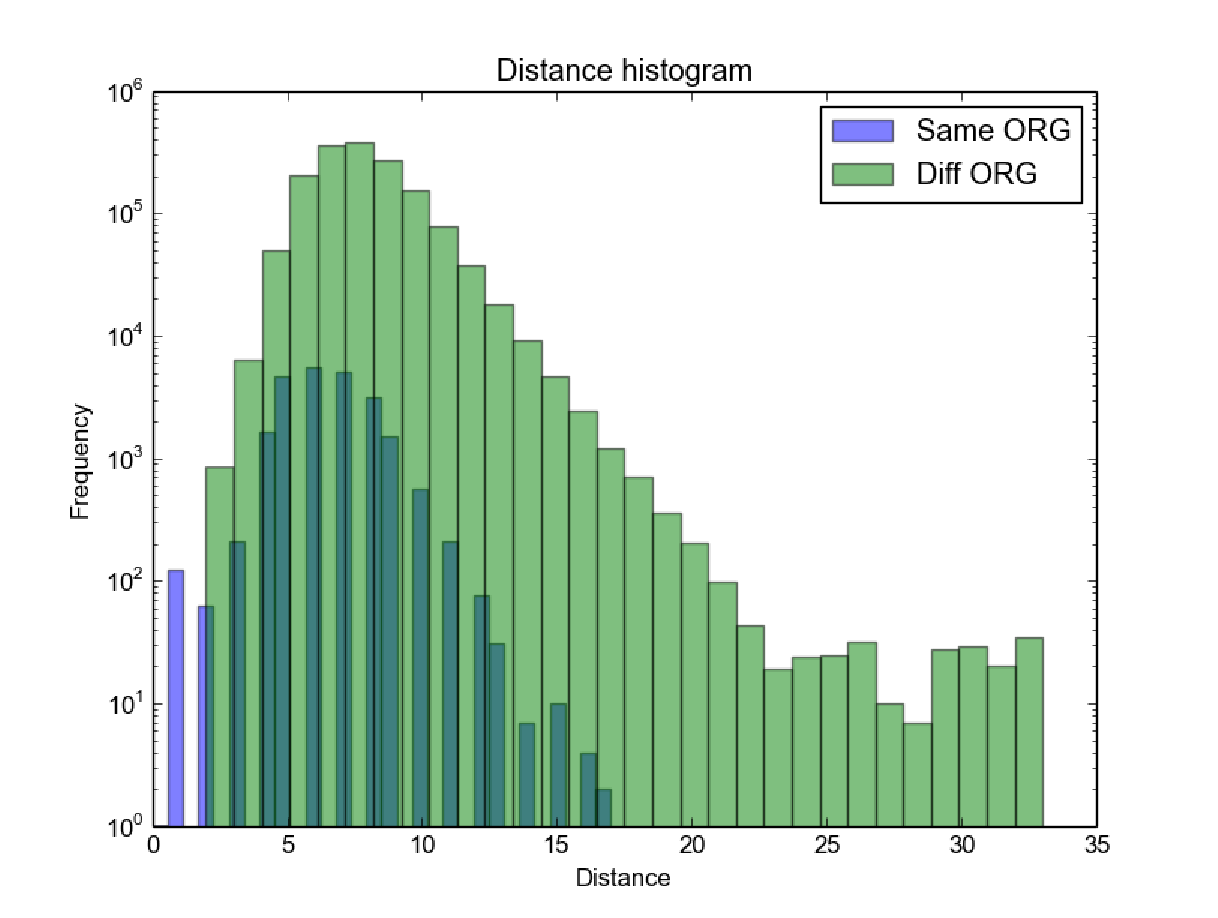
\includegraphics[scale=0.425]{figure/same_diff_org.pdf}
  \caption{ Relationship graph of organisation of an inventor and his distance from Kia Silverbrook}
\label{fig:same_diff}
\end{figure}

\paragraph{Answer 2.}
We divide each inventor into either same 
or different organization. An inventor belongs to 
 same organization category if he has patent with any of the organizations that are 
assignees for Kia Silverbrook's patents. All other inventors fall in the different
organization category. With this division, 
we plot a graph as shown in Figure~\ref{fig:same_diff}.
From the graph, we observe that inventors from same organization have
smaller collaborative distance which is expected. However, interesting observation is that
even many inventors from different organizations have smaller collaborative distance to Kia Silverbrook. 
This answers our Question 2:
Inventors are not only closely connected to an impactful
inventor in their own organization but also in other organizations.



\begin{table}[t]
\centering
\begin{tabular}{|l|c|c|}
\hline
\textbf{Organization}        & \multicolumn{1}{l|}{\textbf{24/7 Wall St}} & \multicolumn{1}{l|}{\textbf{SSL 3.0}} \\ \hline
IBM Corp                     & 1                                          & 1                                         \\ \hline
Samsung Electronics          & 2                                          & 19                                        \\ \hline
Canon K K                    & 3                                          & 4                                         \\ \hline
Sony Corp                    & 4                                          & 13                                        \\ \hline
Microsoft Corp               & 5                                          & 18                                        \\ \hline
\end{tabular}
\caption{Comparison of Rankings by 24/7 Wall St vs. SSL 3.0.}
\label{tab:validation}
\end{table}


\begin{table}[t]
\centering

		\begin{tabular}{| l | l |}
		\hline
		
		{Type} & {Count or Details} \\
		\hline
		\hline
		G1 Nodes & $3421276$ \\
		G1 Edges & $13153732$ \\
		G2 Nodes & $10842560$ \\
		G2 Edges & $53527305$ \\
		G1 Source Node & Kia Silverbrook \\
		Infinite dist. within Org & $6217$\\
		Infinite dist. outside Org& $1817586$ \\
		Patents with zero citations & $1349956$ \\
		\hline
	\end{tabular}		
	\caption { Details of the co-authorship graph}
	\label{tab:model}
\end{table}	

\begin{table}[t]
\centering

	\begin{tabular}{| l | l |}
		\hline
		{Algorithm} & {Time (sec)} \\
		\hline
		\hline
		Bellman-Ford & $0.80$ \\
		Dijkstra & $1.28$ \\
		Johnson & $1.29$ \\
		\hline
	\end{tabular}
	\caption { Performance of the three shortest path algorithms}
	\label{tab:algos}
\end{table}		

\begin{figure}[t]
  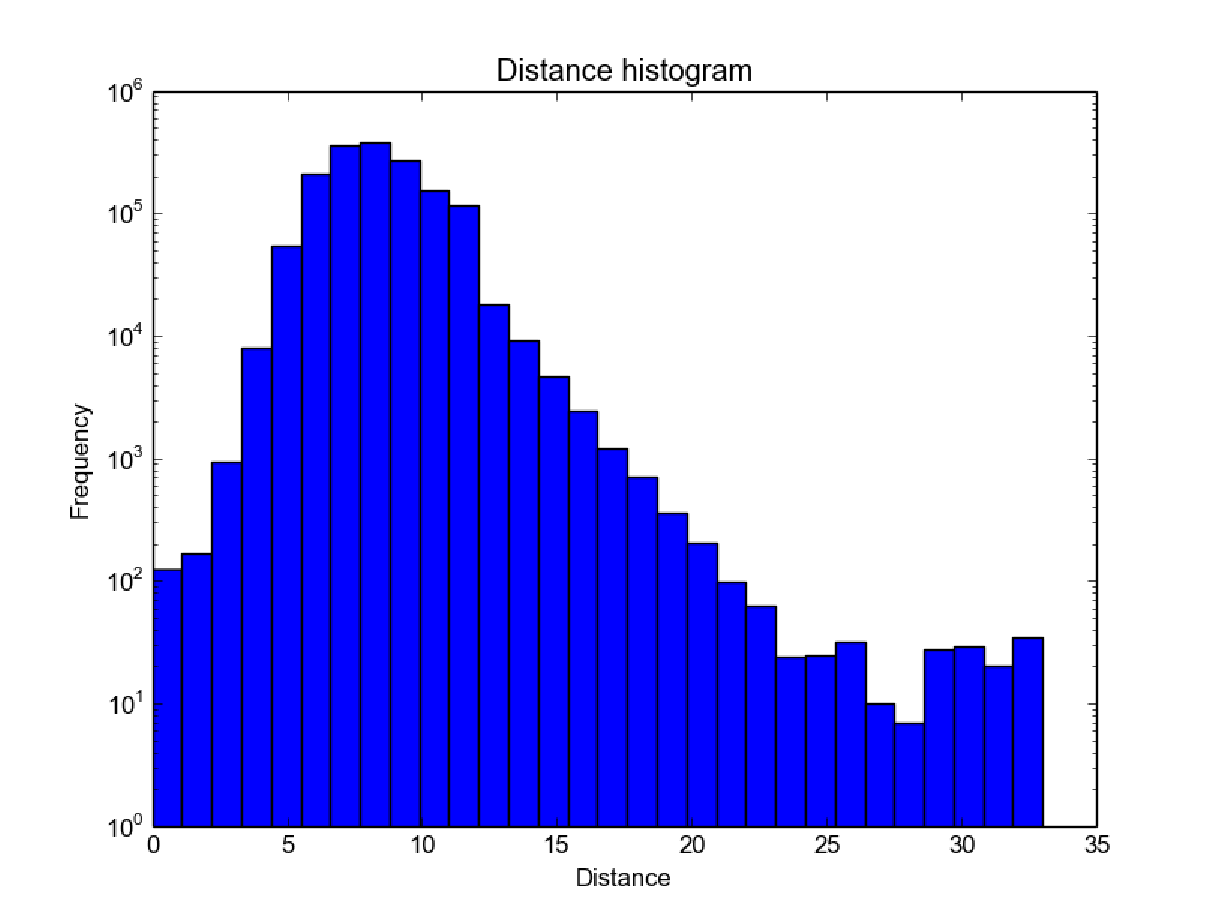
\includegraphics[scale=0.425]{figure/silver_brook_distance.pdf}
  \caption{ Graph shows the frequency of nodes on Y-axis and the distance from
Kia Silverbrook on X-axis }
\label{fig:distance}
\end{figure}

\begin{figure}
  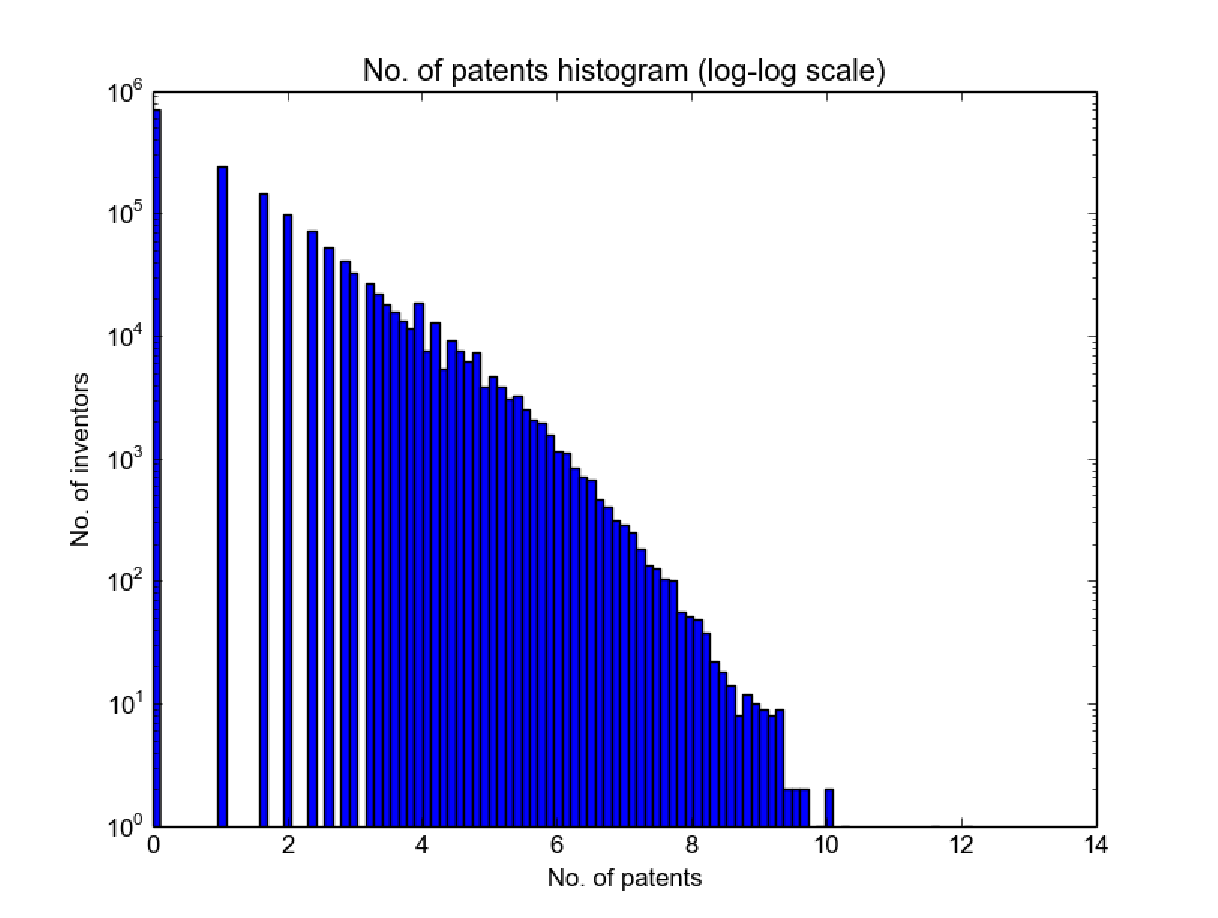
\includegraphics[scale=0.425]{figure/silver_log_log.pdf}
  \caption{ Log-log scale graph of no. of patents on Y-axis and the no.of inventors on X-axis}
\label{fig:patent}	
\end{figure}

\begin{figure}[t]
  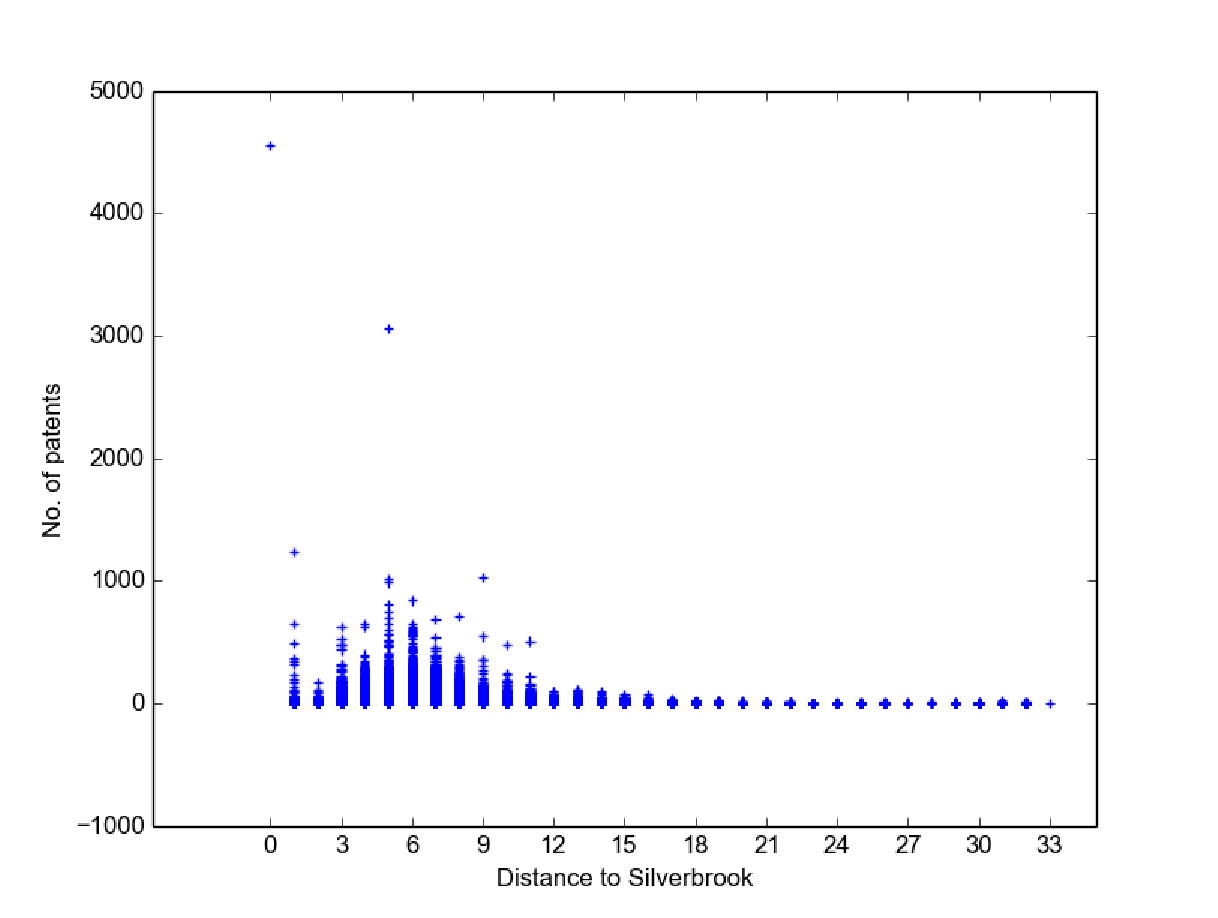
\includegraphics[scale=0.425]{figure/distance_patents.pdf}
  \caption{Relationship graph of no. of patents of an inventor and his distance from Kia Silverbrook}
\label{fig:distance_patent}
\end{figure}

\paragraph{Answer 3.}
We calculate the total number of citations for all patents assigned to a particular organization using graph G2. We rank the organizations based on this metric of total number of citations. Table~\ref{tab:top20} shows the top 20 organisations that are leading the innovation industry via impactful inventions in last four decades, as per our metric. 
This answers our Q3. 

\paragraph{Validating Answer 3.}
To validate the soundness of our proposed metrics, we cross-check our rankings
with public ally available rankings for the year 2013 by 24/7 Wall Street and
Reuters. These two lists are representatives of quantity and quality
respectively.  24/7 Wall Street report is purely based on number of patents
granted to an organization till that year.  On the other hand, Reuters
consider both quantitative as well as qualitative factors with respect to
time. Specifically, the factors such as volume of patents filed in last five
years, success ratio of filed patents, global contributions apart from US
patents, and citation impact of invention in last five years~\cite{reuters-method}.

Table~\ref{tab:validation} shows the top 5 innovative organizations in 2013 as
reported by 24/7 Wall Street and the corresponding rankings as per our
proposed metrics. We report that all of these 5 organizations occur in top 20
list as per our metrics (See Table~\ref{lst:top20} for the complete list).
This validates that our metric fairly succeeds in covering the quantitative
aspects of innovation.

We also compare our rankings to the list of top 100 innovators by Thomas
Reuters. Their report only states the top 100 innovators and does not give any
rankings. Thus, we only compare the percentage of organizations that fall in
top 100 in both Reuters are well as our rankings. On analysis, we find that
this intersection size is 41\%, which validates that our metric fairly
succeeds in covering the qualitative aspects of innovation.


\subsection{Miscellaneous Results}
\paragraph{Graph Details.}
\paragraph{Performance Comparison.}
\paragraph{Collaborative Distance Characteristics.}
\paragraph{Distribution of Quantitative Innovation Impact.}


% \paragraph{Co-inventorGraph Characteristics.}

Table~\ref{tab:algos} shows the execution time for each of the three shortest
path algorithms  when run on our graph G1. We observe that Djikstra's
algorithm takes $1.28$ seconds, Bellman-ford takes $0.80$ seconds and Johnson
algorithm takes $1.29$ seconds to run on our experimental setup.
Figure~\ref{fig:distance} shows the result for the total number of inventors
having the same distance from Kia Silverbrook. Figure~\ref{fig:patent} shows the log-log graph of the total
no.of patents to total no.of inventors. 
Figure~\ref{fig:distance_patent} shows the relation of the distance from
Kia Silverbrook and the no. of patents for an inventor. 




% References:
% http://www.forbes.com/innovative-companies/
% http://top100innovators.com/
% http://www.brw.com.au/lists/50-most-innovative-companies/2014/


% {
% \footnotesize
\bibliography{project}
% }
\end{document}